\chapter{Internet Rzeczy}
%=================================================================================================

\section{Definicja Internetu Rzeczy}
Zgodnie z definicją wskazaną w rekomendacji ITU-T Y.2060, Internet Rzeczy został określony jako ,,globalna infrastruktura dla społeczeństwa, umożliwiająca działanie zaawansowanym serwisom poprzez połączenie (fizyczne i wirtualne) przedmiotów bazujących na istniejących i ewoluujących interoperacyjnych technologiach komunikacji i wymiany informacji''\cite{itu:iot}.

W praktycznym aspekcie, powyższa definicja określa Internet Rzeczy jako złożone systemy udostępniające zaawansowane usługi poprzez komunikację i współpracę różnych urządzeń z wykorzystaniem rozmaitych mediów transmisyjnych, jak np. Internet.

\section{Dziedziny powiązane z konstrukcją i działaniem modułów IoT}
Moduły Internetu Rzeczy stanowią produkt działań specjalistów z wielu branż. Pomijając gałęzie nauki i przemysłu związane bezpośrednio z przeznaczoną funkcjonalnością konkretnego systemu, wyodrębnić można następujące dziedziny, których obecność można uniwersalnie zaobserwować w trakcie analizy różnych systemów.

\begin{itemize}
    \item [$\bullet$] \textbf{Systemy wbudowane} -- leżą one u podstaw oferowanych przez moduły IoT funkcjonalności. Każde z urządzeń wchodzące w skład omawianych sieci musi być wyposażone w układy cyfrowe umożliwiające pełnienie postawionych jemu zadań, takich jak np. dokonywanie pomiarów lub monitorowanie parametrów pracy innego urządzenia. Do ich realizacji wykorzystywane są mikrokontrolery sterujące urządzeniami peryferyjnymi (takimi jak czujniki, wyświetlacze, itp.), wykonujące wstępne przetwarzanie danych (ang. \emph{preprocessing}), oraz umożliwiające komunikację z urządzeniem za pośrednictwem interfejsów komunikacyjnych (wliczając w to interfejsy szeregowe -- np. SPI, I$^2$C -- jak i interfejsy sieciowe).
    
    \newpage
    \item [$\bullet$] \textbf{Analiza danych} -- jednym z głównych zadań modułów sieci IoT jest zbieranie i generowanie danych, które następnie muszą zostać przetworzone przez jednostki o większej mocy obliczeniowej. W zależności od ilości danych oraz wymagań czasowych co do ich prędkości przetwarzania, krok ten jest realizowany na różnych poziomach hierarchii systemu. W celu filtracji, zorganizowania oraz wnioskowania na podstawie danych szeroko używane są formuły matematyczne i algorytmy, które pozwalają m.in. na zebranie powiązanych ze sobą informacji oraz przedstawienie ich w sposób umożliwiający wyciągnięcie głębszej konkluzji.
    
    \item [$\bullet$] \textbf{Sztuczna inteligencja} -- twór bazujący na matematycznych zasadach analizy danych mający na celu znaczne przyspieszenie i automatyzację przetwarzania danych w sposób naśladujący biologiczną inteligencję. Pozwala ona na interpretację ogromnych ilości informacji, w czasie znacznie przekraczającym możliwości całych zespołów ludzi. Przekłada się to na znaczne poprawienie sprawności systemów IoT. Ponadto, sztuczna inteligencja niejednokrotnie stanowi integralną część funkcjonalności dostępnych dla użytkowników, szczególnie w systemach inteligentnych takich jak systemy \emph{smart home} czy systemy zabezpieczeń (np. poprzez możliwość identyfikacji osoby na podstawie danych biometrycznych lub wyglądu). 
    
    \item [$\bullet$] \textbf{Sieci komputerowe} -- ze względu na konieczność wymiany danych pomiędzy urządzeniami leżącą u podstaw koncepcji Internetu Rzeczy, każdy moduł musi być wyposażony w interfejs komunikacyjny lub ich zespół w celu umożliwienia transferu danych zarówno z, jak i do urządzenia. Wspomniane wcześniej interfejsy składają się z interfejsu przewodowego Ethernet albo interfejsów bezprzewodowych WiFi lub GSM. Wymaga to zapewnienia bezpieczeństwa poprzez stosowanie techniki szyfrowania.
    
    \item [$\bullet$] \textbf{Druk 3D} -- moduły IoT często pełnią innowacyjne i niestandardowe zadania, co ogranicza możliwości korzystania z dostępnych na rynku elementów, jak np. obudowy, elementy mocujące oraz elementy wykonawcze ruchomych mechanizmów. Ogromną przewagą odznacza się tutaj branża druku 3D pozwalająca na bardzo szybkie i łatwe przygotowanie elementów prototypowych oraz elementów dla finalnego produktu znacząco zmniejszając koszty produkcji.
\end{itemize}
    
\section{Główne zalety oraz wady}
    Systemy Internetu Rzeczy są innowacyjną i bardzo elastyczną techniką, dzięki czemu charakteryzują się szeregiem zalet, spośród których najważniejszymi są:
    
    \begin{itemize}
        \item [$\bullet$] stanowienie przestrzeni do innowacyjnych pomysłów wpływających zarówno na standard życia społeczeństwa, jak i wydajność przemysłu oraz badań naukowych;
        \item [$\bullet$] zapewnianie większego bezpieczeństwa obiektów oraz personelu, co jest szczególnie istotne w miejscach pracy o podwyższonym ryzyku;
        \item [$\bullet$] umożliwienie monitorowania zmian zachodzących w otoczeniu pod wpływem różnych czynników i upływu czasu;
        \item [$\bullet$] gromadzenie wartościowych danych pomiarowych, które są zbyt obszerne lub niemożliwe do wykrycia bezpośrednio przez człowieka (np. ustalenie konkretnego poziomu zanieczyszczenia powietrza).
    \end{itemize}
    
    Duża część zaprezentowanych zalet wynika z metodyki konstruowania modułów i projektowania systemów Internetu Rzeczy wykorzystującej różnorodne elementy o szerokim wachlarzu zastosowań do konstrukcji układów przeznaczonych do ściślej określonych zadań. Jako przykład można wskazać dostępne systemy typu \emph{smart home}, które przy użyciu elementów takich jak czujniki wilgoci, czujniki dymu i czujniki drgań są w stanie nadzorować bezpieczeństwo domu (zarówno chroniąc przed pożarem, jak i np. włamaniem).
    
    Podobnie, jak w przypadku wszystkich technologii, systemy IoT nie mogą obejść się bez wad wynikających z obecnego stopnia zaawansowania technologicznego, jakości komponentów, czy też założeń projektowych tworzonych rozwiąząń. Największe z nich to:
    
    \begin{itemize}
        \item [$\bullet$] mocno ograniczona moc obliczeniowa końcowych urządzeń pomiarowych, wymuszająca połączenie z centralnym punktem o znacznie większej mocy w celu przetworzenia dużych pakietów danych;
        \item [$\bullet$] wymóg zakupu zestawu urządzeń w celu utworzenia kompletnego, w pełni funkcjonalnego systemu, co zniechęca klientów indywidualnych;
        \item [$\bullet$] konieczność obsługi komunikacji z wieloma urządzeniami oddalonymi od siebie na zróżnicowane odległości (niekiedy bardzo duże, szczególnie w przypadku systemów o przeznaczeniu przemysłowym i środowiskowym).
    \end{itemize}
    
    Stosunek wad do zalet rozwiązań Internetu Rzeczy jest kwestią dyskusyjną i w pełni zależną od konkretnych przypadków zastosowań.


%=================================================================================================
\section{Moduły IoT jako urządzenia sieci Internet}

Sieć Internet stanowi bardzo popularne medium transmisyjne w wielu domach, biurach oraz budynkach przemysłowych. Jej koncepcja -- stanowiąca jedną z podstaw dziedziny Internetu Rzeczy -- sprawiła, że większość modułów IoT obecnie wykorzystuje dostęp do Internetu jako fundament systemu, którego są częścią. Szczególnie zauważalne jest to w przypadku systemów przeznaczonych dla klientów indywidualnych oraz firm biurowych.

W celu komunikacji z wykorzystaniem Internetu, moduły IoT posiadają potrzebę implementacji stosu komunikacyjnego bazującego na modelu OSI (ang. \emph{Open System Interconnection Reference Model}) autorstwa Międzynarodowej Organizacji Normalizacyjnej ISO (ang. \emph{International Organization for Standarization}). Stanowi on 7{\dywiz}warstwową hierarchię elementów systemu komunikacyjnego z podziałem ze względu na pełnione role. Zgodnie z treścią prezentacji autorstwa pracownika Katedry Inteligentnych Systemów Informatycznych Politechniki Częstochowskiej profesora nadzwyczajnego Roberta Nowickiego \cite{kisi:osi} poszczególne warstwy modelu OSI (począwszy od najwyższej) pełnią następujące funkcje:

\begin{itemize}
    \item [1)] warstwa aplikacji -- odpowiada za standardowe funkcjonalności programów, takie jak m.in. przeglądanie stron WWW, oraz zapewnia wspólne API dla różnorodnych usług;
    \item [2)] warstwa prezentacji -- pełni funkcję formatowania danych do ogólnie udostalonej postaci wykorzystującej zdefiniowaną składnię;
    \item [3)] warstwa sesji -- powiadamia użytkownika o błędach występujących w niższych warstwach, zapewnia synchronizację i zarządzanie sesjami pomiędzy usługami;
    \item [4)] warstwa transportowa -- nadzoruje połączenia występujące w warstwie sieciowej, powiązane z nimi zdarzenia jak np. upływ czasu przetwarzania (ang. \emph{timeout}) oraz prawidłowość przesyłu sekwencji pakietów;
    \item [5)] warstwa sieciowa -- pełni funkcje adresacji sieci, podziału i scalania pakietów na fragmenty, a także podejmuje decyzję o trasie którą pakiety zostaną przesłane;
    \item [6)] warstwa łącza danych -- zajmuje się tworzeniem ramki transmisyjnej, określaniem zasad transmisji i nadzorowaniem przebiegu wymiany danych w warstwie fizycznej;
    \item [7)] warstwa fizyczna -- pełni rolę fizycznego medium przesyłu danych.
\end{itemize}

Na podstawie powyższego modelu utworzony został stos protokołów komunikacyjnych TCP/IP, w którym warstwy aplikacji, prezentacji oraz sesji zostały nazwane zbiorczo warstwą aplikacji, a warstwy łącza danych i fizyczna zostały połączone w warstwę interfejsu sieciowego, tworząc hierarchię 4{\dywiz}warstwową. Na każdym poziomie wyróżnić można grupę protokołów odpowiedzialnych za przystosowanie nadawanych danych do transmisji, tzw. enkapsulację (ang. \emph{encapsulation}), oraz przetworzenie otrzymanych danych z postaci ramki transmisyjnej na postać użyteczną dla usługi końcowej (np. przeglądarki internetowej) \cite{techdifferences:ositcpip}. Graficzne porównanie warstw obu modeli przedstawione zostało na rysunku 2.1.

\begin{figure}[!ht]
    \centering
    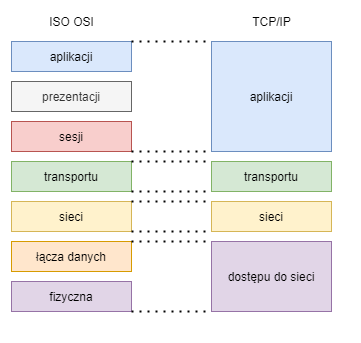
\includegraphics[width=80mm]{Praca/Rysunki/Rozdzial2/iso_osi_vs_tcp.png}
    \caption{Graficzne porównanie modeli ISO OSI oraz TCP/IP}
    \label{fig:my_label}
\end{figure}